\chapter{Feedback}

\textit{Feedback} is for evaluated teams to evaluate the \textit{Peer Evaluations} they have received and it is also a very important component in determining whether the evaluator team can pass or not. After realizing the lack of extensibility in the design for \textit{PeerEvaluations} and with more time available for implementation of \textit{Feedback}, a Survey Template and question creation system has been set up, which made the system open for extensions for more questions and even question types.

\section{Survey Template and question creation system}

The basic flow when a request to create a \textit{Feedback} is illustrated in the figure below:

\begin{figure}[h]
    \centering
    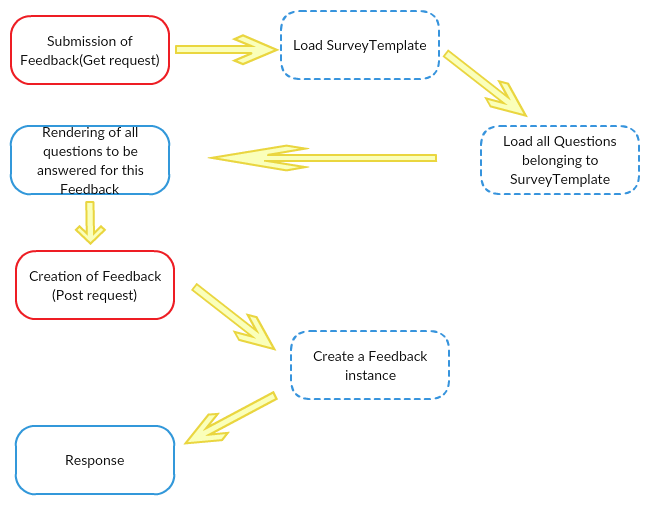
\includegraphics[width=0.5\textwidth]{Images/Skylab_Feedback_Flow.png}
    \caption{Flow of a feedback creation process}
\end{figure}

So when a student clicks the button to create feedback, \textit{FeedbacksController}'s \textit{new} action will be invoked and inside the method, the corresponding \textit{SurveyTemplate} and all \textit{Questions} belonging to the SurveyTemplate will be sent to view. Then instruction for the \textit{Feedback} and all questions will be rendered as response to the student. After the student completed and pressed submit button, responses to all questions will be sent to server and a Feedback instance containing all submitted responses will be created.

There currently 3 types of \textit{Questions} in the system:

\begin{itemize}
  \item \textbf{TextQuestion}: a text question which will be rendered in the format of textarea and text-based responses are expected. 
  \item \textbf{RichTextQuestion}: a rich text question which will be rendered in the format of TinyMCE editable area and rich text is expected as response.
  \item \textbf{MultipleChoiceQuestion}: a multiple choice question which will be rendered as checkboxes followed by option descriptions and one option value is expected.
\end{itemize}

\begin{figure}[h]
    \centering
    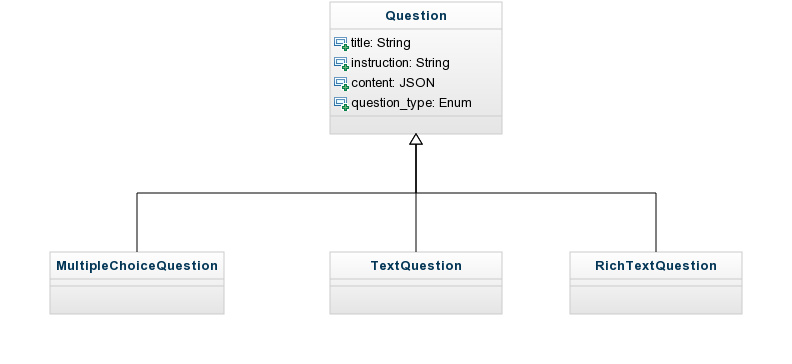
\includegraphics[width=0.85\textwidth]{Images/Skylab_Questions.jpg}
    \caption{3 types of questions in Skylab}
\end{figure}

Each type of question will have its own way of rendering and validation. In this way, adding new types of questions can simply be done via creating a new question model with its own rendering and validation.
